% Going off the Thesis guidelines available here: http://www.lboro.ac.uk/students/welcome/research/codes-of-practice/appendices/
% A4 paper size selected, default is 11pt font, to change to 12pt use [a4paper, 12pt] as option to documentclass
\documentclass[a4paper]{report}

% Some useful packages for including images, colored font, etc.
\usepackage[dvips]{graphicx}
\graphicspath{{Figures/}}

\makeatletter
\def\maxwidth{\ifdim\Gin@nat@width>\linewidth\linewidth\else\Gin@nat@width\fi}
\def\maxheight{\ifdim\Gin@nat@height>\textheight\textheight\else\Gin@nat@height\fi}
\makeatother
\setkeys{Gin}{width=\maxwidth,height=\maxheight,keepaspectratio}
\usepackage{amssymb,amsmath}
\usepackage{longtable}
\usepackage{booktabs}

\usepackage{listings}
\usepackage{xcolor}
 
\definecolor{codegreen}{rgb}{0,0.6,0}
\definecolor{codegray}{rgb}{0.5,0.5,0.5}
\definecolor{codepurple}{rgb}{0.58,0,0.82}
\definecolor{backcolour}{rgb}{0.95,0.95,0.92}
 
\lstdefinestyle{mystyle}{
    backgroundcolor=\color{backcolour},   
    commentstyle=\color{codegreen},
    keywordstyle=\color{magenta},
    numberstyle=\tiny\color{codegray},
    stringstyle=\color{codepurple},
    basicstyle=\ttfamily\footnotesize,
    breakatwhitespace=false,         
    breaklines=true,                 
    captionpos=b,                    
    keepspaces=true,                 
    numbers=left,                    
    numbersep=5pt,                  
    showspaces=false,                
    showstringspaces=false,
    showtabs=false,                  
    tabsize=2
}
 
\lstset{style=mystyle}

\usepackage[numbers]{natbib}

\usepackage{color}
\usepackage{url}
% Used for subfigures
\usepackage{subcaption}
% Used for landscape pages
\usepackage{pdflscape}
% Used for hyper-links in contents, etc.
\usepackage[hidelinks]{hyperref}
\hypersetup{
    linktoc=all
}

% Global bibliography style
\bibliographystyle{unsrt}

% Set margins in all document to 3.5cm as per guidelines for binding
\usepackage[includeheadfoot,margin=3.5cm]{geometry}

% Used to including pdf files within pages
% use [draft] as option to output empty spaces rather than rendering all pages (useful when including lots of pdfs)
\usepackage{pdfpages}

% Used to produce headers and footers
\usepackage{fancyhdr}
\pagestyle{fancyplain}

% Used for removing title in bibliography sections
\usepackage{titlesec}

% Used to generate lists of abbreviations
\usepackage{nomencl}
\makenomenclature 
\renewcommand{\nomname}{List of Abbreviations} 

% To have a separate bibliography per Chapter uncomment this line
% See Introduction/Introduction.tex for example how to include the bibliography
%\usepackage{chapterbib}

% Line spacing defined at 1 and a half. I know it says 1.3 but its 1 and a half.
\linespread{1.3}

% Setup headers and footers
\fancyhf{}
\lhead{\leftmark}
% Center on all pages
% \fancyhead[C]{---Draft---}
% Page number placed on right side on odd pages and left side on even pages
\fancyfoot[RO, LE] {\thepage}


\begin{document}

% Give \subsubsection numbers
\setcounter{secnumdepth}{4}

% Title, Author, Abstract, Acknowledgement, Table of Content, List of Figures, List of Tables and List of Abbreviations
% Front matter of the Thesis
% Title page
% Loughborough University Thesis Access Form
% Loughborough University Certificate of Originality
% Abstract
% Acknowledgements
\title{\bf Image Compression Simulation}

\author{by\\Zhihao DAI\\
\\
{\bf COP501 Advanced Programming}\\
{\bf Coursework Report}\\
\\
Loughborough University\\
\\
\copyright
\hspace{1 dd} Zhihao DAI 2019\\
\\
Nov. 2019
}
\date{} % Used to remove date from title so it can be set at any date rather than the current date

\maketitle

% Set page numbers to roman numerals for front matter
\pagenumbering{roman}

% % PDF exports of Word Documents available (Exported August 2012)
% % Thesis Access Form
% 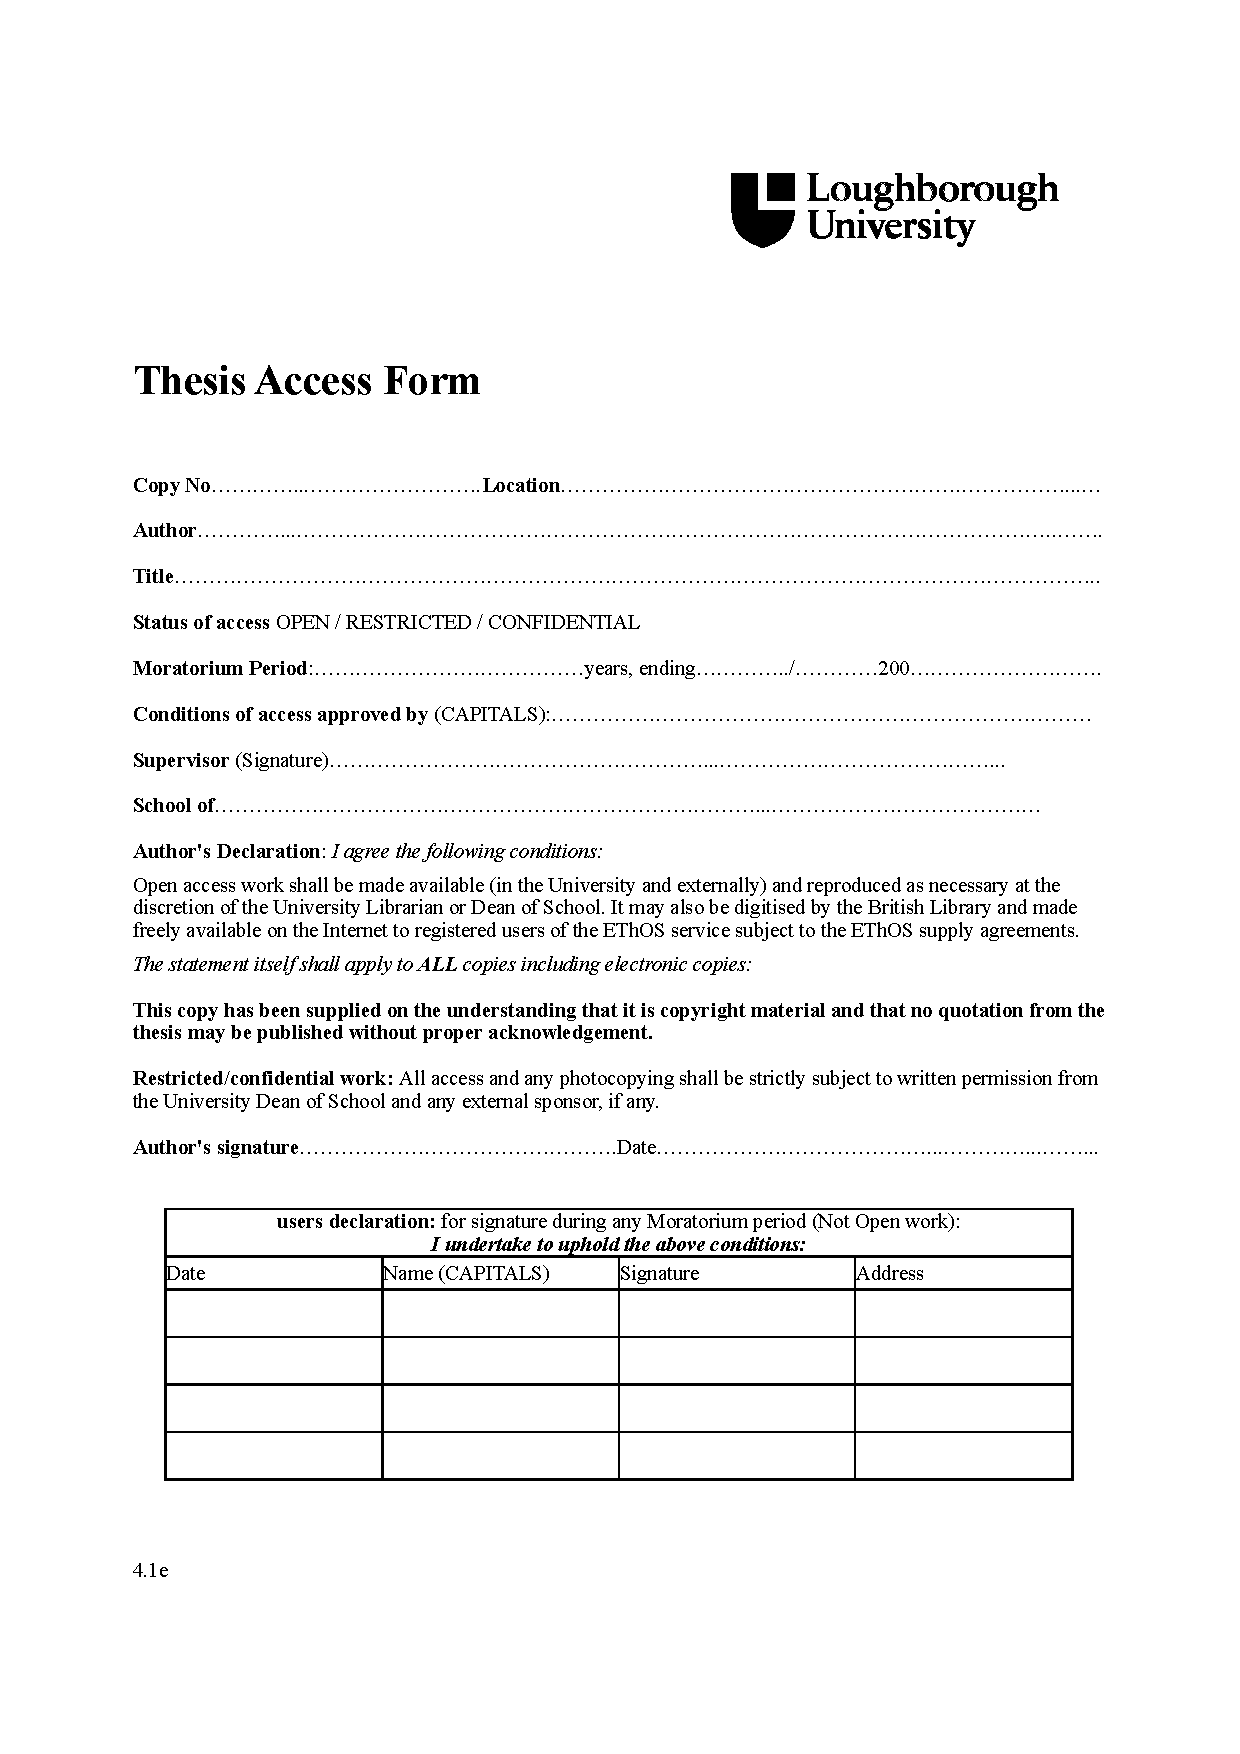
\includepdf[pages=1, pagecommand=, templatesize={5in}{10in}]{Front/LU/access.pdf}
% % Certificate of Originality
% 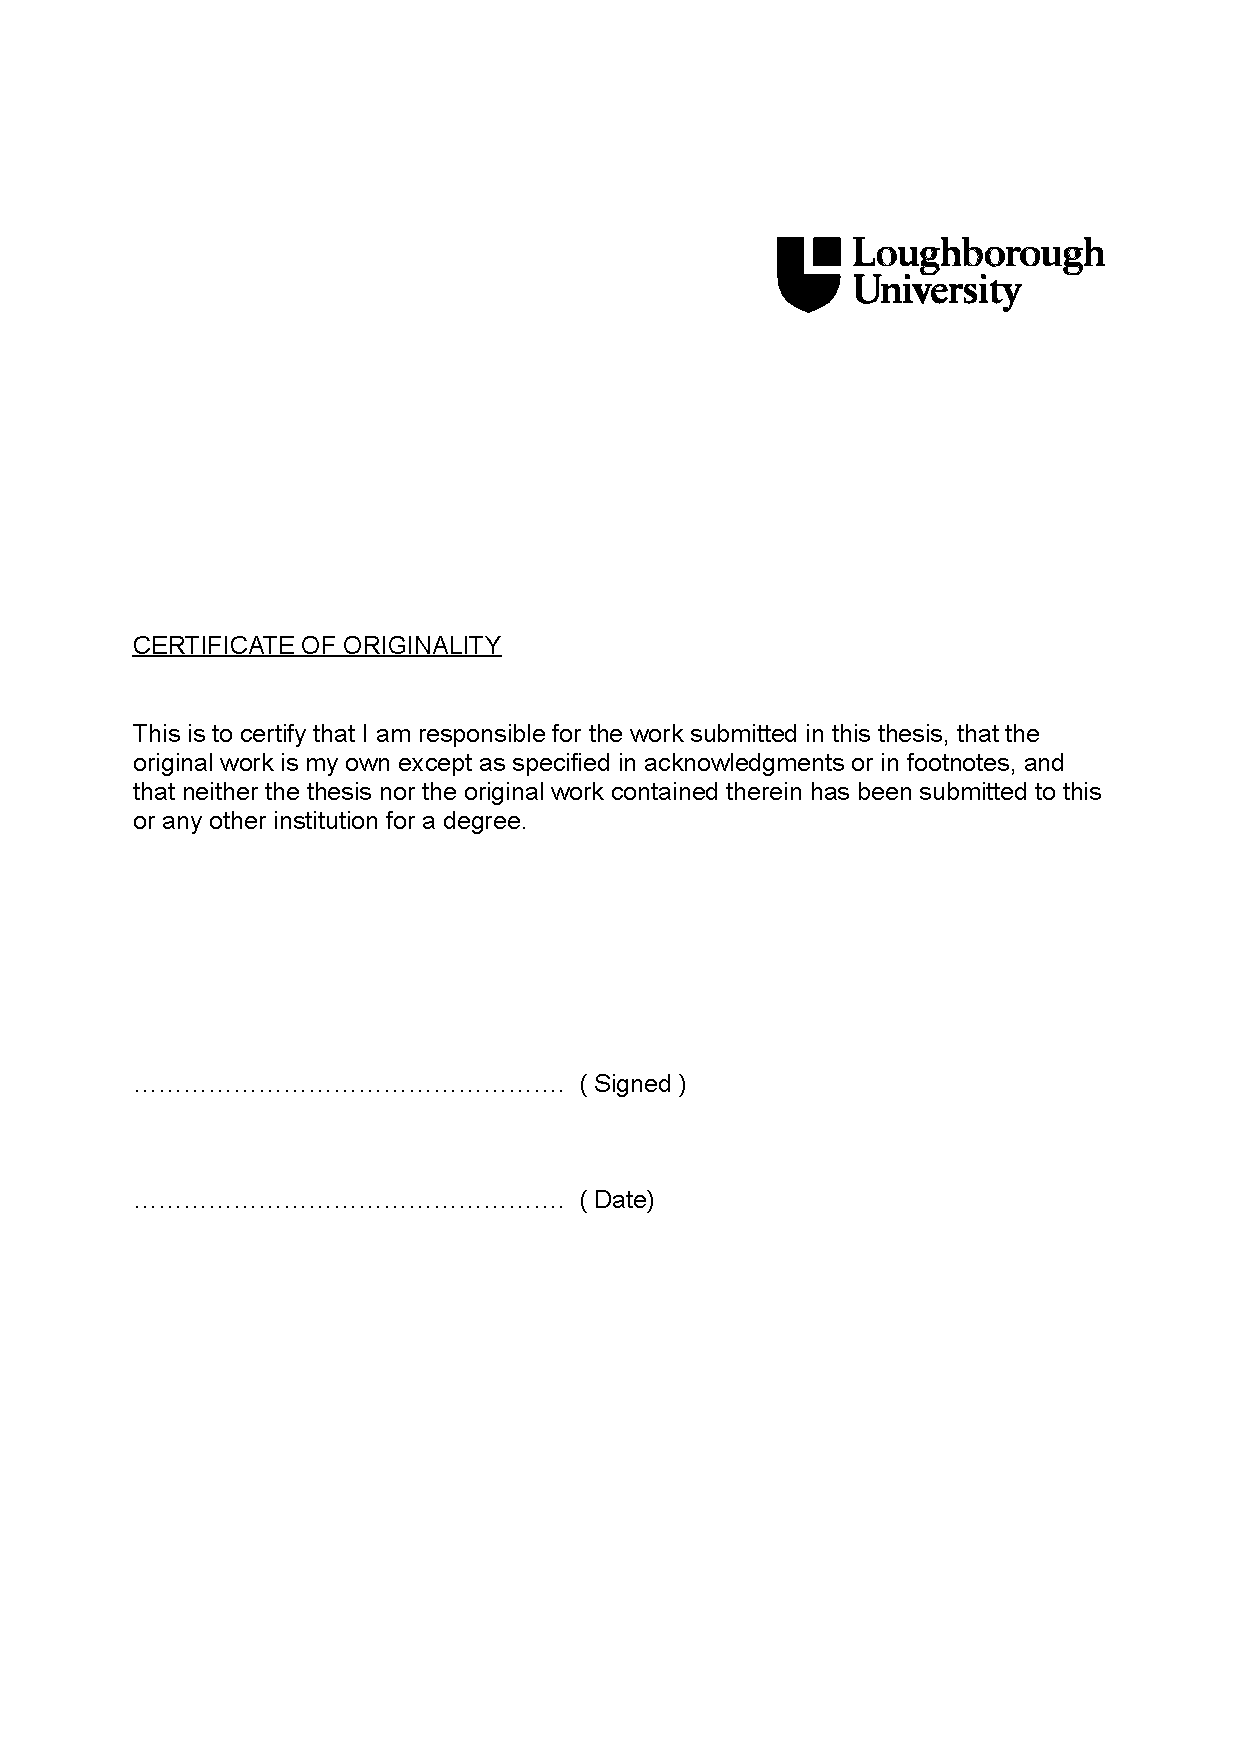
\includepdf[pages=-, pagecommand=, templatesize={5in}{10in}]{Front/LU/origin.pdf}

% Abstract
\addcontentsline{toc}{chapter}{Abstract}
\chapter*{Abstract}
In this coursework, I implement a JPEG Image Compression Simulation using MATLAB as frontend GUI and Python as backend JPEG CODEC. There are 2 simulation parameters $K$ and $Q'$ in the application. 
Several specific design considerations are introduced to the implementation, inclding an end-to-end MATLAB interface, an "Video Compression" functionality and DCT as Matrix Computation.
I conclude that both $K$ and $Q'$ can significantly affect the quality of the compressed image.


% % Acknowledgements
% \addcontentsline{toc}{chapter}{Acknowledgements}
% \chapter*{Acknowledgements}
% Acknowledgement section.

% Set the depth for your table of content
% Currently set at 2 (Chapter, Section, Subsection)
\setcounter{tocdepth}{2}
% Include a table of content
\tableofcontents

% Include a list of figures
\addcontentsline{toc}{chapter}{List of Figures}
\listoffigures

% Include a list of tables
\addcontentsline{toc}{chapter}{List of Tables}
\listoftables

% Include a list of Listings
\addcontentsline{toc}{chapter}{List of Listings}
\renewcommand*{\lstlistlistingname}{List of Listings}
\lstlistoflistings

% Include a list of abbreviations using nomenclature package
%\addcontentsline{toc}{chapter}{List of Abbreviations}
%\printnomenclature[3cm] 

\newpage

% Set page numbering to arabic for body of Thesis
\pagenumbering{arabic}


% To keep everything neat I included each chapter as a separate .tex file
% Each contains a single chapter, they include all the settings defined in this .tex file
% Allows easier moving around of chapters

% Use \include{<path to .tex file>} to include documents
% For example
\chapter{Introduction}
\label{chap:introduction}

\section{Image Compression}

Image compression is to decrease the size of the image file without dramatically downgarding the quality of the image.

In this courework, I set out to implement a simulation of the JPEG (Joint Photographic Experts Group) image compression process\citep{wallace1992jpeg}. The implementation uses MATLAB as frontend interface and Python as backend.

\section{JPEG Standard}

The JPEG Still Picture Compression Standard is widely used on modern digital devices, ranging from computers, cameras to smartphones. For a grayscale image, a JPEG CODEC (Encoder and Decoder) typically involves 6 main steps as illustrated in Figure \ref{fig:codec}.

\begin{figure}
\centering
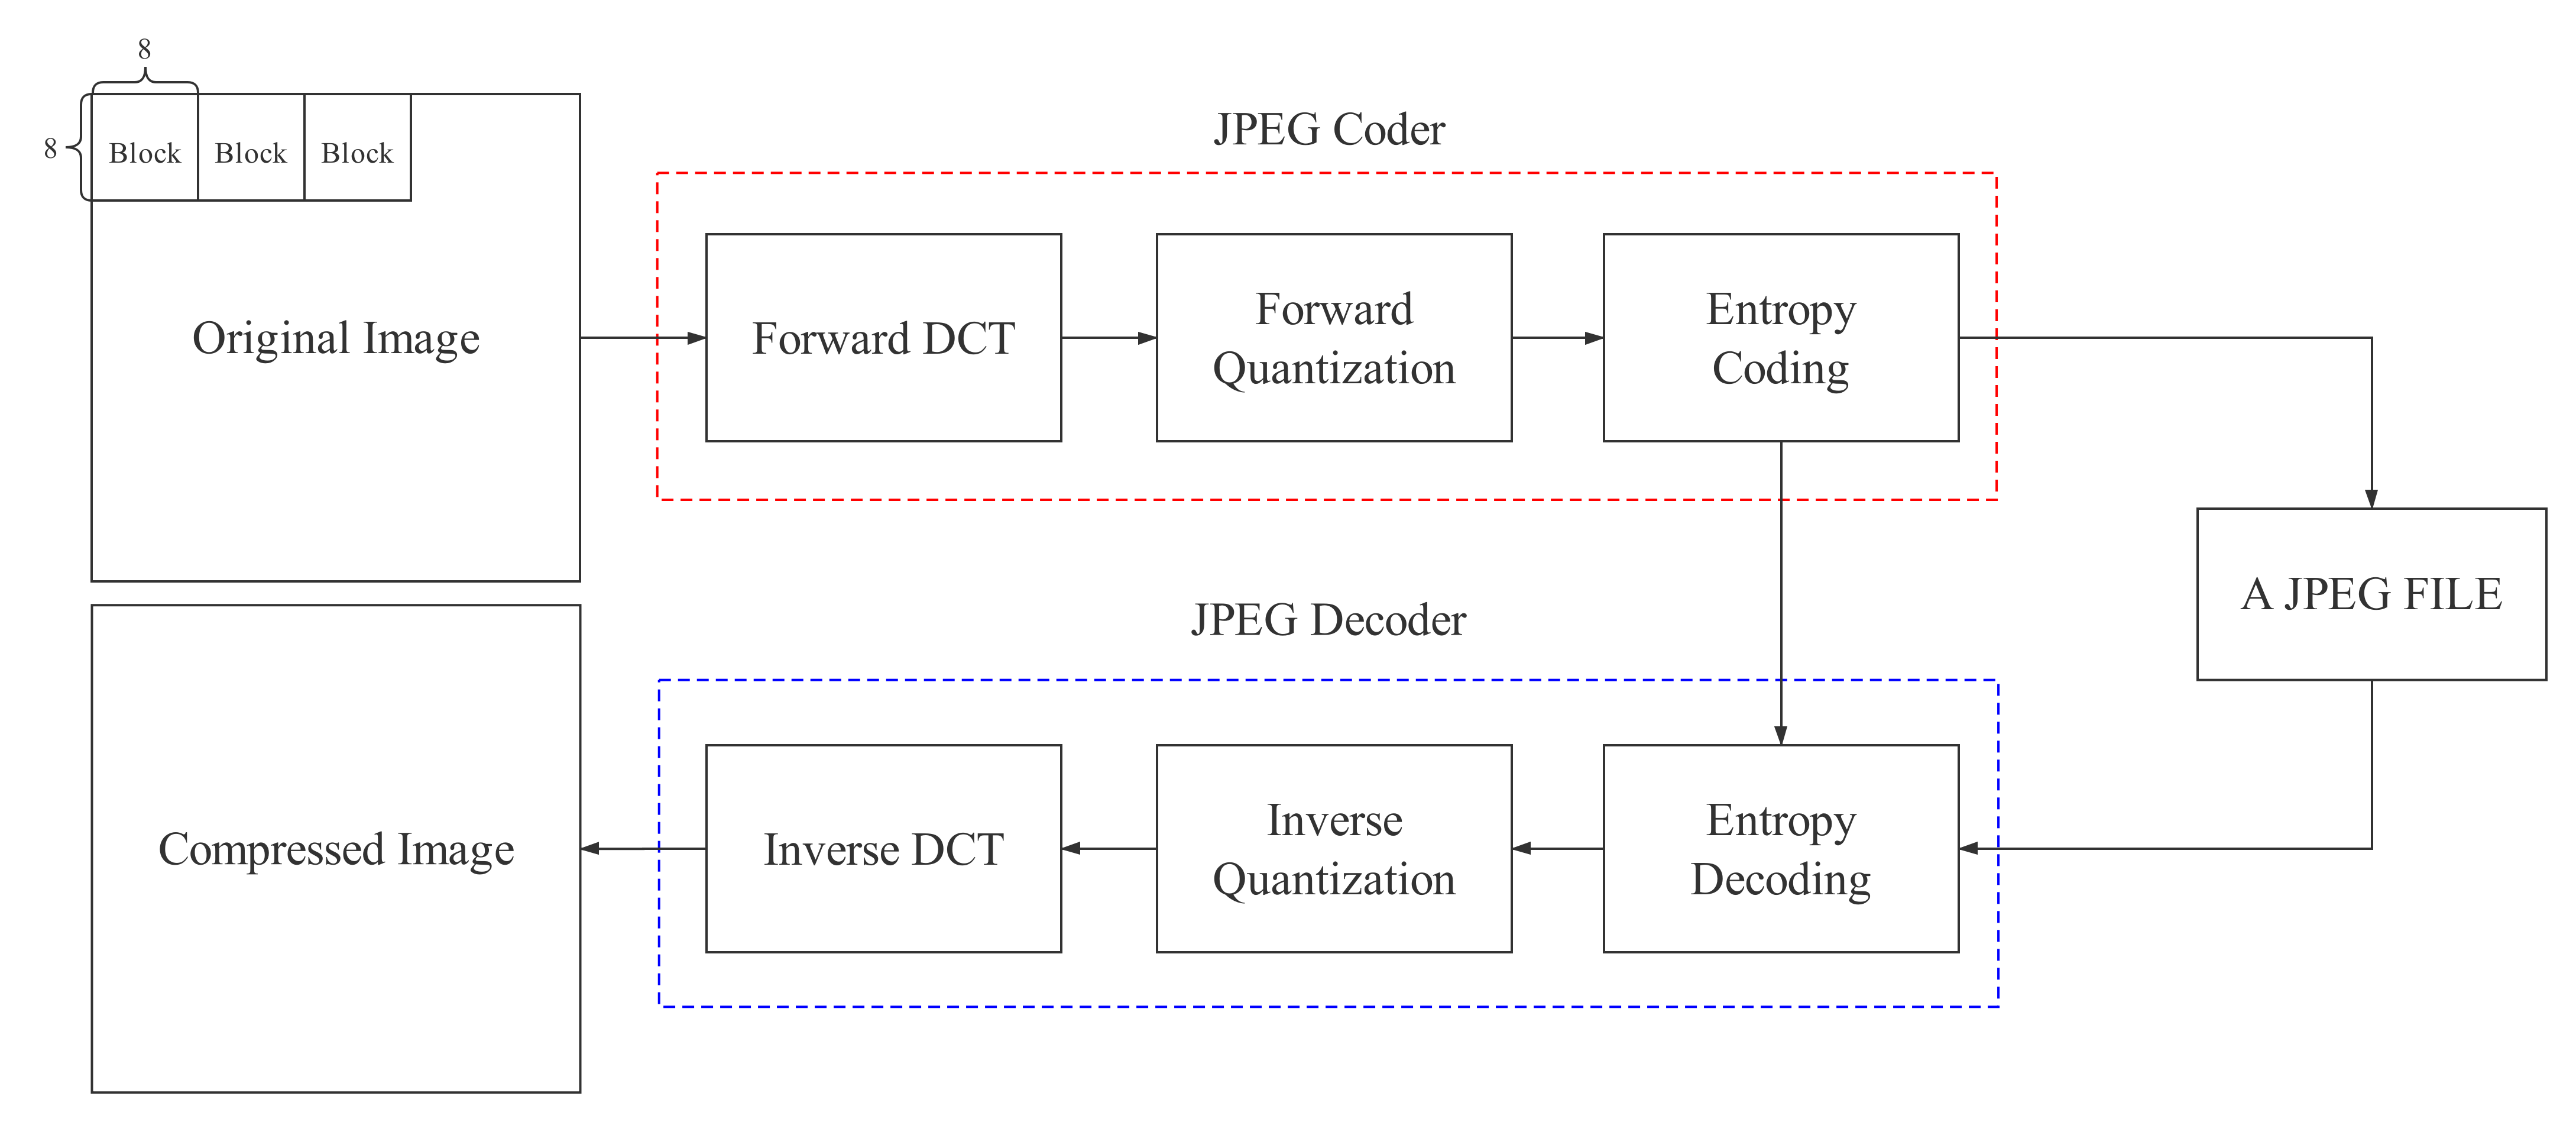
\includegraphics{codec}
\caption{Six Main Steps of a JPEG CODEC.}
\label{fig:codec}
\end{figure}

In my application, I implement a simplified JPEG CODEC in Python programming language. The CODEC consists of both foward and inverse steps of Discrete Cosine Transform (DCT) and Quantization and gets rid of both forward and inverse steps of Entropy Coding. 

Since Entropy Codeing is reversible through Inverse Entropy Coding and does not affect the quality of the image, my implementation should be able to simulate the full effects of JPEG coding on any given still image despite its simplicity.

As shown in Figure \ref{fig:app}, given an input grayscale image in uint8 matrix format, the application first crops the image array to multiply of $8$ in both column (width) and row (height). Then, a value of $128$ is subtracted from the image for each pixel value. After that, the matrix is divided into 8 by 8 blocks. Each block then goes through FDCT, Quantization, Inverse Quantization and IDCT individually.  All resulted blocks are placed in their previous position and a new matrix is thus formed. Finally, a value of $128$ is added back to the new matrix to get the compressed grayscale image. 

\begin{figure}
\centering
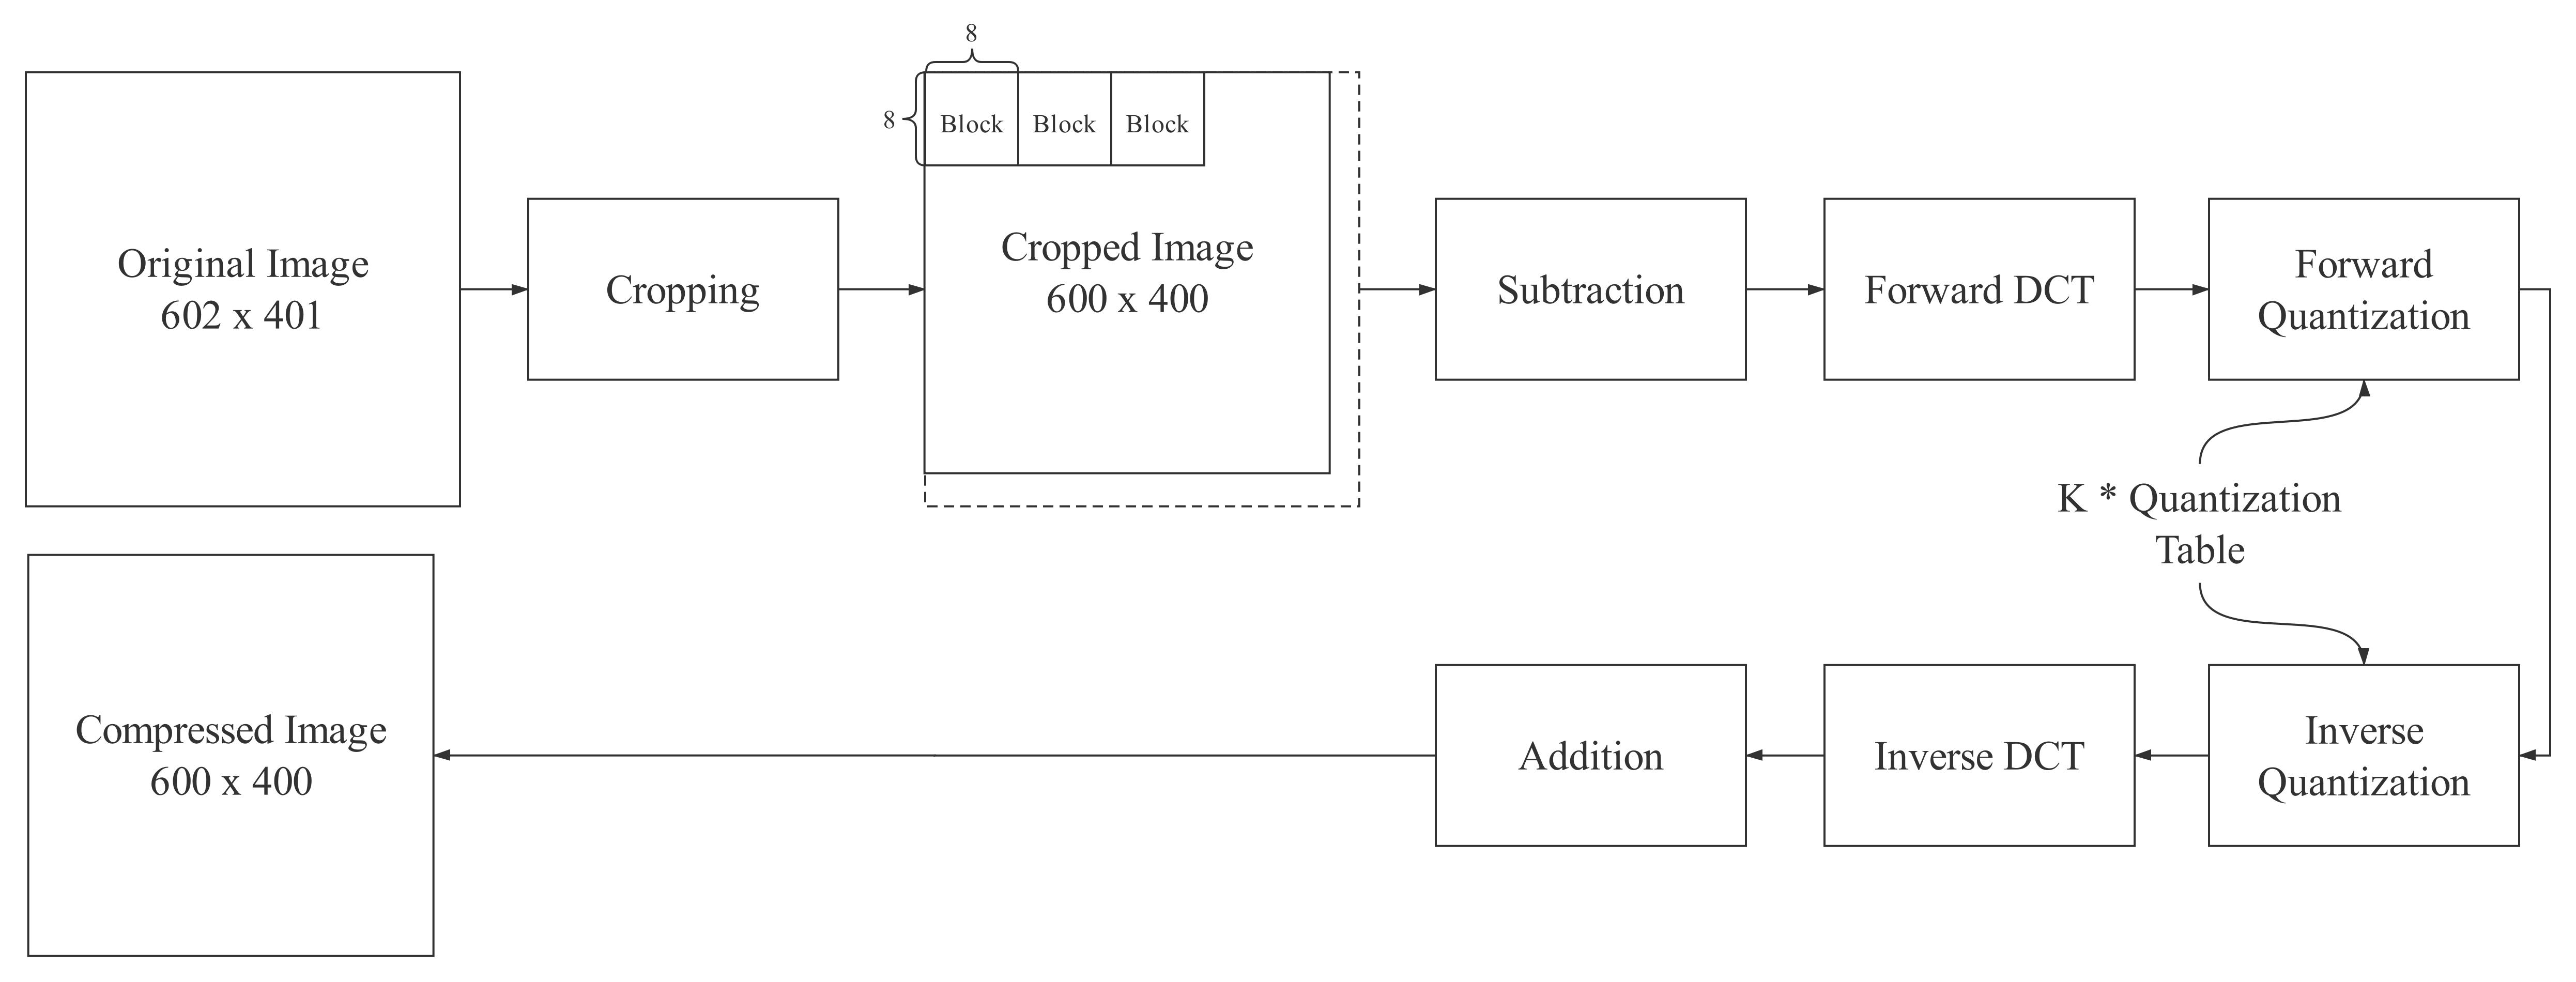
\includegraphics{app}
\caption{Main Steps of the Application.}
\label{fig:app}
\end{figure}

For a color RGB image, the same process is carried out on each color channel respectively.

\subsection{Discrete Cosine Transform (DCT)}

The forward step of DCT is computed using the following equation.

\begin{equation}
F(u, v) = \frac{1}{4} C(u) C(v) [\sum_{x=0}^7 \sum_{y=0}^7 f(x,y) * cos\frac{(2x+1)u\pi}{16} cos\frac{(2y+1)v\pi}{16}]
\label{equ:fdct}
\end{equation}

where $C(t) = 1/\sqrt(2)$ for $t = 0$; $C(t) = 1$ otherwise. Both input $f$ and output $F$ is an 8 by 8 block.

The inverse step of DCT is computed using the following equation.

\begin{equation}
f(x, y) = \frac{1}{4} [\sum_{u=0}^7 \sum_{v=0}^7 C(u) C(v) F(u, v) * cos\frac{(2x+1)u\pi}{16} cos\frac{(2y+1)v\pi}{16}]
\label{equ:idct}
\end{equation}

where $C(t) = 1/\sqrt(2)$ for $t = 0$; $C(t) = 1$ otherwise. Both input $F$ and output $f$ is an 8 by 8 block.

\subsection{Quantization}

The forward step of Quantization is computed using the following equation.

\begin{equation}
F^Q(u, v) = round(\frac{F(u, v)}{Q(u, v)})
\label{equ:fq}
\end{equation}

where $Q$ is the Quantization Table specified in the JPEG standard. Both input $F$ and ouput $F^Q$ is an 8 by 8 block.

The inverse step of Quantization is computed using the following equation.

\begin{equation}
F(u, v) = F^Q(u, v) * Q(u, v))
\label{equ:iq}
\end{equation}

where $Q$ should be the same as in the forward step. Both input $F^Q$ and ouput $F$ is an 8 by 8 block.

By default, the value of $Q$ is specfied as followed.

\begin{equation}
Q = 
\begin{bmatrix}
  16& 11& 10& 16& 24& 40& 51& 61 \\
  12& 12& 14& 19& 26& 58& 60& 55 \\
  14& 13& 16& 24& 40& 57& 69& 56 \\
  14& 17& 22& 29& 51& 87& 80& 62 \\
  18& 22& 37& 56& 68& 109& 103& 77 \\
  24& 35& 55& 64& 81& 104& 113& 92 \\
  49& 64& 78& 87& 103& 121& 120& 101 \\
  72& 92& 95& 98& 112& 100& 103& 99
\end{bmatrix}
\label{equ:q}
\end{equation}








\chapter{More Examples}
\label{chap:examples}

\section{Subfigures}
\begin{figure*}[ht!]
    \centering
    \begin{subfigure}[b]{0.67\textwidth}
        \centering
        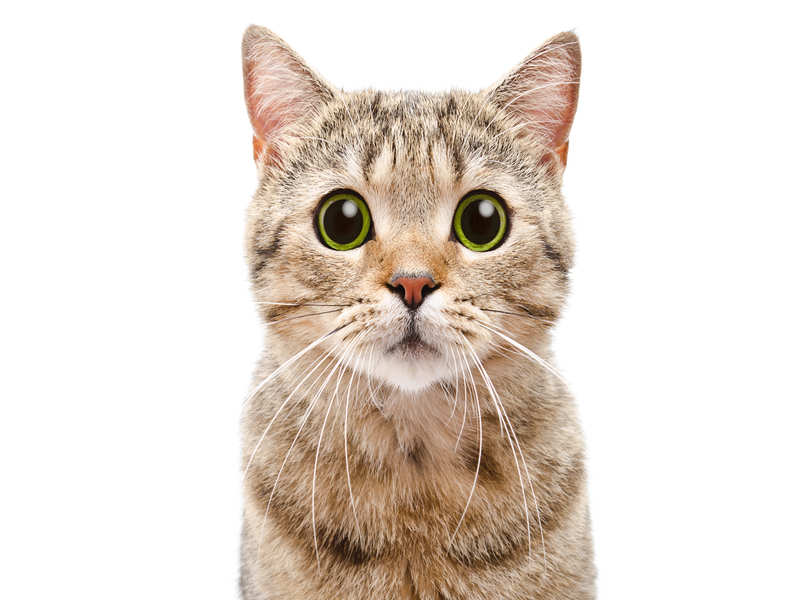
\includegraphics[width=\linewidth]{cat}
        \caption{Figure 1}
    \end{subfigure}
    \hfill
    \begin{minipage}[b]{0.3\textwidth}
	    \begin{subfigure}[b]{\linewidth}
	        \centering
	        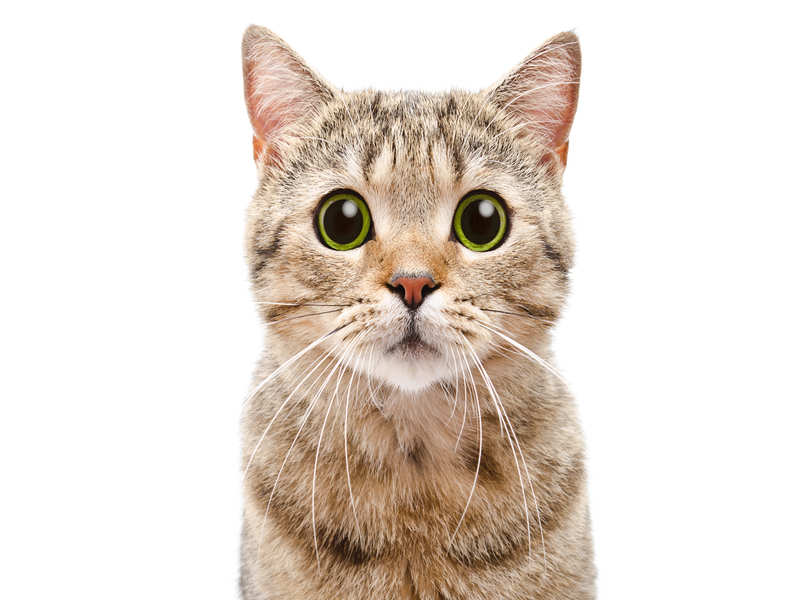
\includegraphics[width=\linewidth]{cat}
	        \caption{Figure 2}
	    \end{subfigure}
	    \\
	    \begin{subfigure}[b]{\linewidth}
	        \centering
	        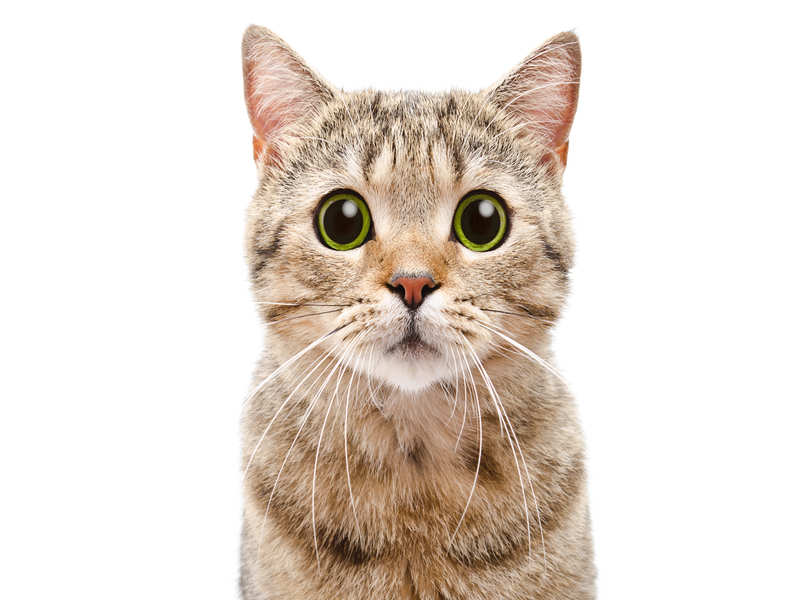
\includegraphics[width=\linewidth]{cat}
	        \caption{Figure 3}
	    \end{subfigure}
	\end{minipage}
    \caption{Subfigures in One Figure (1).}
    \label{fig:subfigures-1}
\end{figure*}

\begin{figure*}[ht!]
    \centering
    \begin{subfigure}[b]{0.67\textwidth}
        \centering
        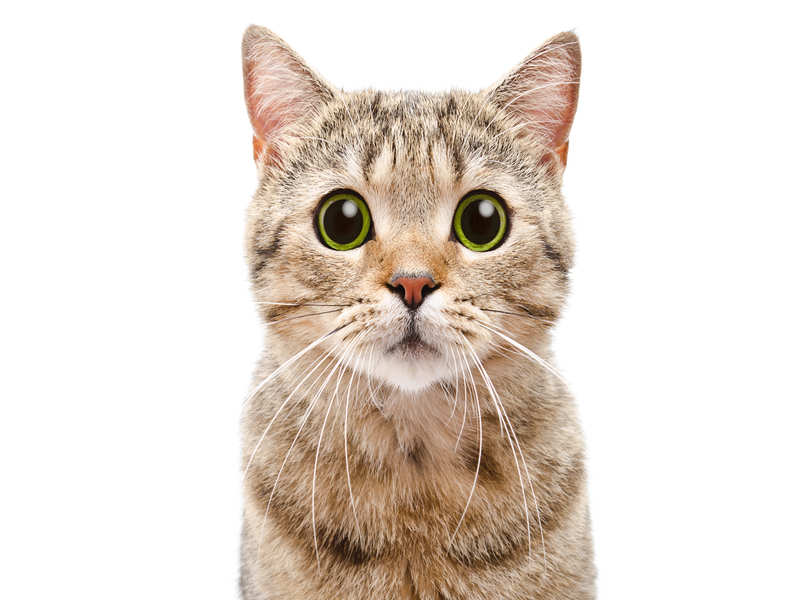
\includegraphics[width=\linewidth]{cat}
        \caption{Figure 1}
    \end{subfigure}
    ~
    \begin{subfigure}[b]{0.67\textwidth}
        \centering
        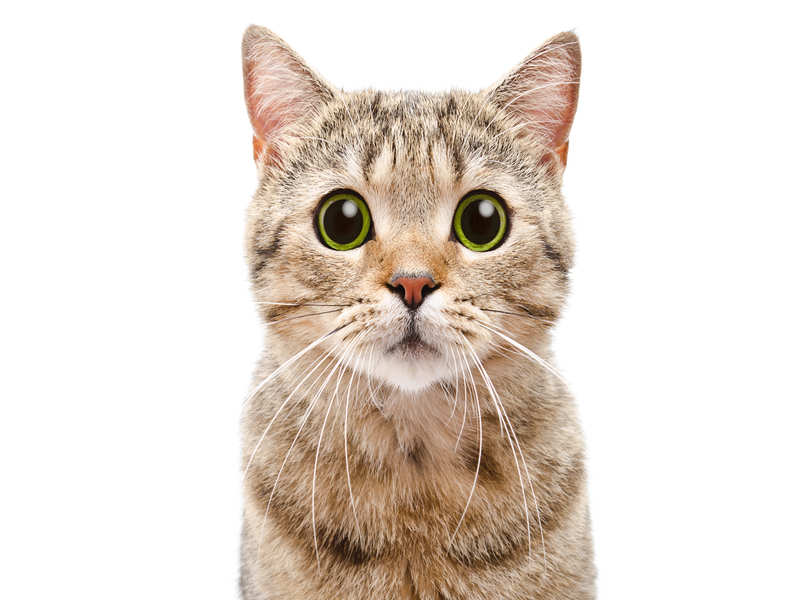
\includegraphics[width=\linewidth]{cat}
        \caption{Figure 2}
    \end{subfigure}
    \caption{Subfigures in One Figure (2).}
    \label{fig:subfigures-2}
\end{figure*}

\section{Landscape Page}

\begin{landscape}
\scriptsize{
\begin{longtable}[]{@{}lllll@{}}
\toprule
Subnet & IPv4 Address / Prefix & IPv4 Address Range & IPv6
Address / Prefix & IPv6 Address Range\tabularnewline
\midrule
\endhead
\texttt{BT-R001} - \texttt{BT001} & \texttt{23.0.0.0/28} &
\texttt{23.0.0.1} - \texttt{23.0.0.14} & \texttt{2001:2300:0:0::/64} &
\texttt{2001:2300:0:0::1} -
\texttt{2001:2300:0:0:ffff:ffff:ffff:fffe}\tabularnewline
\texttt{BT-R002} - \texttt{BT002} & \texttt{23.0.0.16/28} &
\texttt{23.0.0.17} - \texttt{23.0.0.30} & \texttt{2001:2300:0:1::/64} &
\texttt{2001:2300:0:1::1} -
\texttt{2001:2300:0:1:ffff:ffff:ffff:fffe}\tabularnewline
\texttt{BT-R003} - \texttt{BT003} & \texttt{23.0.0.32/28} &
\texttt{23.0.0.33} - \texttt{23.0.0.62} & \texttt{2001:2300:0:2::/64} &
\texttt{2001:2300:0:2::1} -
\texttt{2001:2300:0:2:ffff:ffff:ffff:fffe}\tabularnewline
\texttt{BT-R001} - \texttt{BT-R002} & \texttt{23.0.0.48/30} &
\texttt{23.0.0.49} - \texttt{23.0.0.50} & \texttt{2001:2300:0:3::/64} &
\texttt{2001:2300:0:3::1} -
\texttt{2001:2300:0:3:ffff:ffff:ffff:fffe}\tabularnewline
\texttt{BT-R002} - \texttt{BT-R003} & \texttt{23.0.0.52/30} &
\texttt{23.0.0.53} - \texttt{23.0.0.54} & \texttt{2001:2300:0:4::/64} &
\texttt{2001:2300:0:4::1} -
\texttt{2001:2300:0:4:ffff:ffff:ffff:fffe}\tabularnewline
\texttt{BT-R001} - \texttt{BT-R003} & \texttt{23.0.0.56/30} &
\texttt{23.0.0.57} - \texttt{23.0.0.58} & \texttt{2001:2300:0:5::/64} &
\texttt{2001:2300:0:5::1} -
\texttt{2001:2300:0:5:ffff:ffff:ffff:fffe}\tabularnewline
\texttt{BT-R002} - \texttt{DT} & \texttt{23.0.0.60/30} &
\texttt{23.0.0.61} - \texttt{23.0.0.62} & \texttt{2001:2300:0:6::/64} &
\texttt{2001:2300:0:6::1} -
\texttt{2001:2300:0:6:ffff:ffff:ffff:fffe}\tabularnewline
\texttt{BT-R003} - \texttt{Virgin} & \texttt{56.0.0.60/30} &
\texttt{56.0.0.61} - \texttt{56.0.0.62} & \texttt{2001:5600:0:6::/64} &
\texttt{2001:5600:0:6::1} -
\texttt{2001:5600:0:6:ffff:ffff:ffff:fffe}\tabularnewline
\texttt{BT-R003} - \texttt{Central} & \texttt{100.100.2.0/30} &
\texttt{100.100.2.1} - \texttt{100.100.2.2} & &\tabularnewline
\bottomrule
\caption{Allocation of IPv4 and IPv6 Addresses to Subnets in BT Network.}
\label{tab:ip}
\end{longtable}
}

\scriptsize{
\begin{longtable}[]{@{}lllllll@{}}
\toprule
Connection & Interface 1 & IPv4 Address & IPv6 Address & Interface 2 & IPv4 Address & IPv6
Address \tabularnewline
\midrule
\endhead
\texttt{BT-R001} - \texttt{BT001} & \texttt{BT-R001}:
\texttt{FastEthernet0/1/0} & \texttt{23.0.0.1} &
\texttt{2001:2300:0:0::1} & \texttt{BT001}: \texttt{eth0} &
\texttt{23.0.0.2} & \texttt{2001:2300:0:0::2}\tabularnewline
\texttt{BT-R002} - \texttt{BT002} & \texttt{BT-R002}:
\texttt{FastEthernet0/1/0} -\textgreater{} \texttt{Vlan\ 1} &
\texttt{23.0.0.17} & \texttt{2001:2300:0:1::1} & \texttt{BT002}:
\texttt{eth0} & \texttt{23.0.0.18} &
\texttt{2001:2300:0:1::2}\tabularnewline
\texttt{BT-R003} - \texttt{BT003} & \texttt{BT-R003}:
\texttt{FastEthernet0/1/0} -\textgreater{} \texttt{Vlan\ 2} &
\texttt{23.0.0.33} & \texttt{2001:2300:0:2::1} & \texttt{BT003}:
\texttt{eth0} & \texttt{23.0.0.34} &
\texttt{2001:2300:0:2::2}\tabularnewline
\texttt{BT-R001} - \texttt{BT-R002} & \texttt{BT-R001}:
\texttt{FastEthernet0/0} & \texttt{23.0.0.49} &
\texttt{2001:2300:0:3::1} & \texttt{BT-R002}: \texttt{FastEthernet0/0} &
\texttt{23.0.0.50} & \texttt{2001:2300:0:3::2}\tabularnewline
\texttt{BT-R002} - \texttt{BT-R003} & \texttt{BT-R002}:
\texttt{FastEthernet0/1} & \texttt{23.0.0.53} &
\texttt{2001:2300:0:4::1} & \texttt{BT-R003}: \texttt{FastEthernet0/1} &
\texttt{23.0.0.54} & \texttt{2001:2300:0:4::2}\tabularnewline
\texttt{BT-R001} - \texttt{BT-R003} & \texttt{BT-R001}:
\texttt{FastEthernet0/1} & \texttt{23.0.0.57} &
\texttt{2001:2300:0:5::1} & \texttt{BT-R003}: \texttt{FastEthernet0/0} &
\texttt{23.0.0.58} & \texttt{2001:2300:0:5::2}\tabularnewline
\texttt{BT-R002} - \texttt{DT} & \texttt{BT-R002}:
\texttt{FastEthernet0/1/1} -\textgreater{} \texttt{Vlan\ 3} &
\texttt{23.0.0.61} & \texttt{2001:2300:0:6::1} & \texttt{DT} &
\texttt{23.0.0.62} & \texttt{2001:2300:0:6::2}\tabularnewline
\texttt{BT-R003} - \texttt{Virgin} & \texttt{BT-R003}:
\texttt{FastEthernet0/1/2} -\textgreater{} \texttt{Vlan\ 4} &
\texttt{56.0.0.62} & \texttt{2001:5600:0:6::2} & \texttt{Virgin} &
\texttt{56.0.0.61} & \texttt{2001:5600:0:6::1}\tabularnewline
\texttt{BT-R003} - \texttt{Central} & \texttt{BT-R003}:
\texttt{FastEthernet0/1/1} -\textgreater{} \texttt{Vlan\ 5} &
\texttt{100.100.2.2} & & \texttt{Central} & \texttt{100.100.2.1}
&\tabularnewline
\bottomrule
\caption{Interfaces for Each Physical Connection and Corresponding IPv4 and IPv6 Addresses.}
\label{tab:interfaces}
\end{longtable}
}

\end{landscape}

% \include{Chapter/Requirements}
% \include{Chapter/Design}
% \include{Chapter/Testing}
% \include{Chapter/Discussion}

% Include a Chapter names References to the table of content
\addcontentsline{toc}{chapter}{References}
% Rename Bibliography to References
\renewcommand\bibname{References}
\bibliography{Bib/tex}

% Include authors publications and appendix section
% \addcontentsline{toc}{chapter}{Publications}
\chapter*{Publications}
\label{chap:Publications}

% Author publication section
% If not using the references per chapter option you need to include the bibliography inline
% This was done by creating a bibtex file containing the publications and including in a separate LaTeX file, using \nocite{*} this includes all bibtex items, generating the .bbl file and then copying and pasting below.

List of authors academic publications

\begingroup
% Remove title and space of header for this chapter
\titleformat{\chapter}[display]
    {\normalfont\huge\bfseries}{\chaptertitlename\ \thechapter}{20pt}{\Huge}
\titlespacing*{\chapter}{0pt}{0pt}{-80pt}
\renewcommand\bibname{}
\begin{thebibliography}{1}

%\bibitem{}

\end{thebibliography}
\endgroup

% To include copies of the publications use the includepdf package and point to .pdf files of papers
% Example
%\includepdf[pages=-, pagecommand=, templatesize={5in}{10in}]{Publications/Pubs/le1_biothreads.pdf}

% Appedix
\appendix

\begingroup

\chapter{Source Code}
\label{app:code}


\section{JPEG CODEC Code in Python}
\label{app:sec:python}

\subsection{matlab.py}
\lstinputlisting[language=Python]{Code/matlab.py}


\endgroup


\end{document}
